\documentclass{article}
\usepackage{graphicx}
\graphicspath{{/home/li/图片/}}
\usepackage{multicol}
\usepackage{lscape}
\author{Qingyun Li}
\date{April 25, 2018}
\title{Kaggle’s Iceberg Classifier Challenge}
\begin{document}
\maketitle
 \par David Austin, who, with his teammate, took home 1st palce in Kaggle's Iceberg Classify Challenge. Their winning solution can be practically used to allow safer navigation for ships and boats across hazardous waters, resulting in less damages to ships and cargo, and most importantly, reduce accidents, injuries, and deaths. He said that it would be particularly difficult for a humman to accurately predict the classifications, it would serve as a great test to see what computer vision and deep learning could do. 
\begin{figure}[htbp]
\begin{minipage}{1\linewidth}
\centering{}
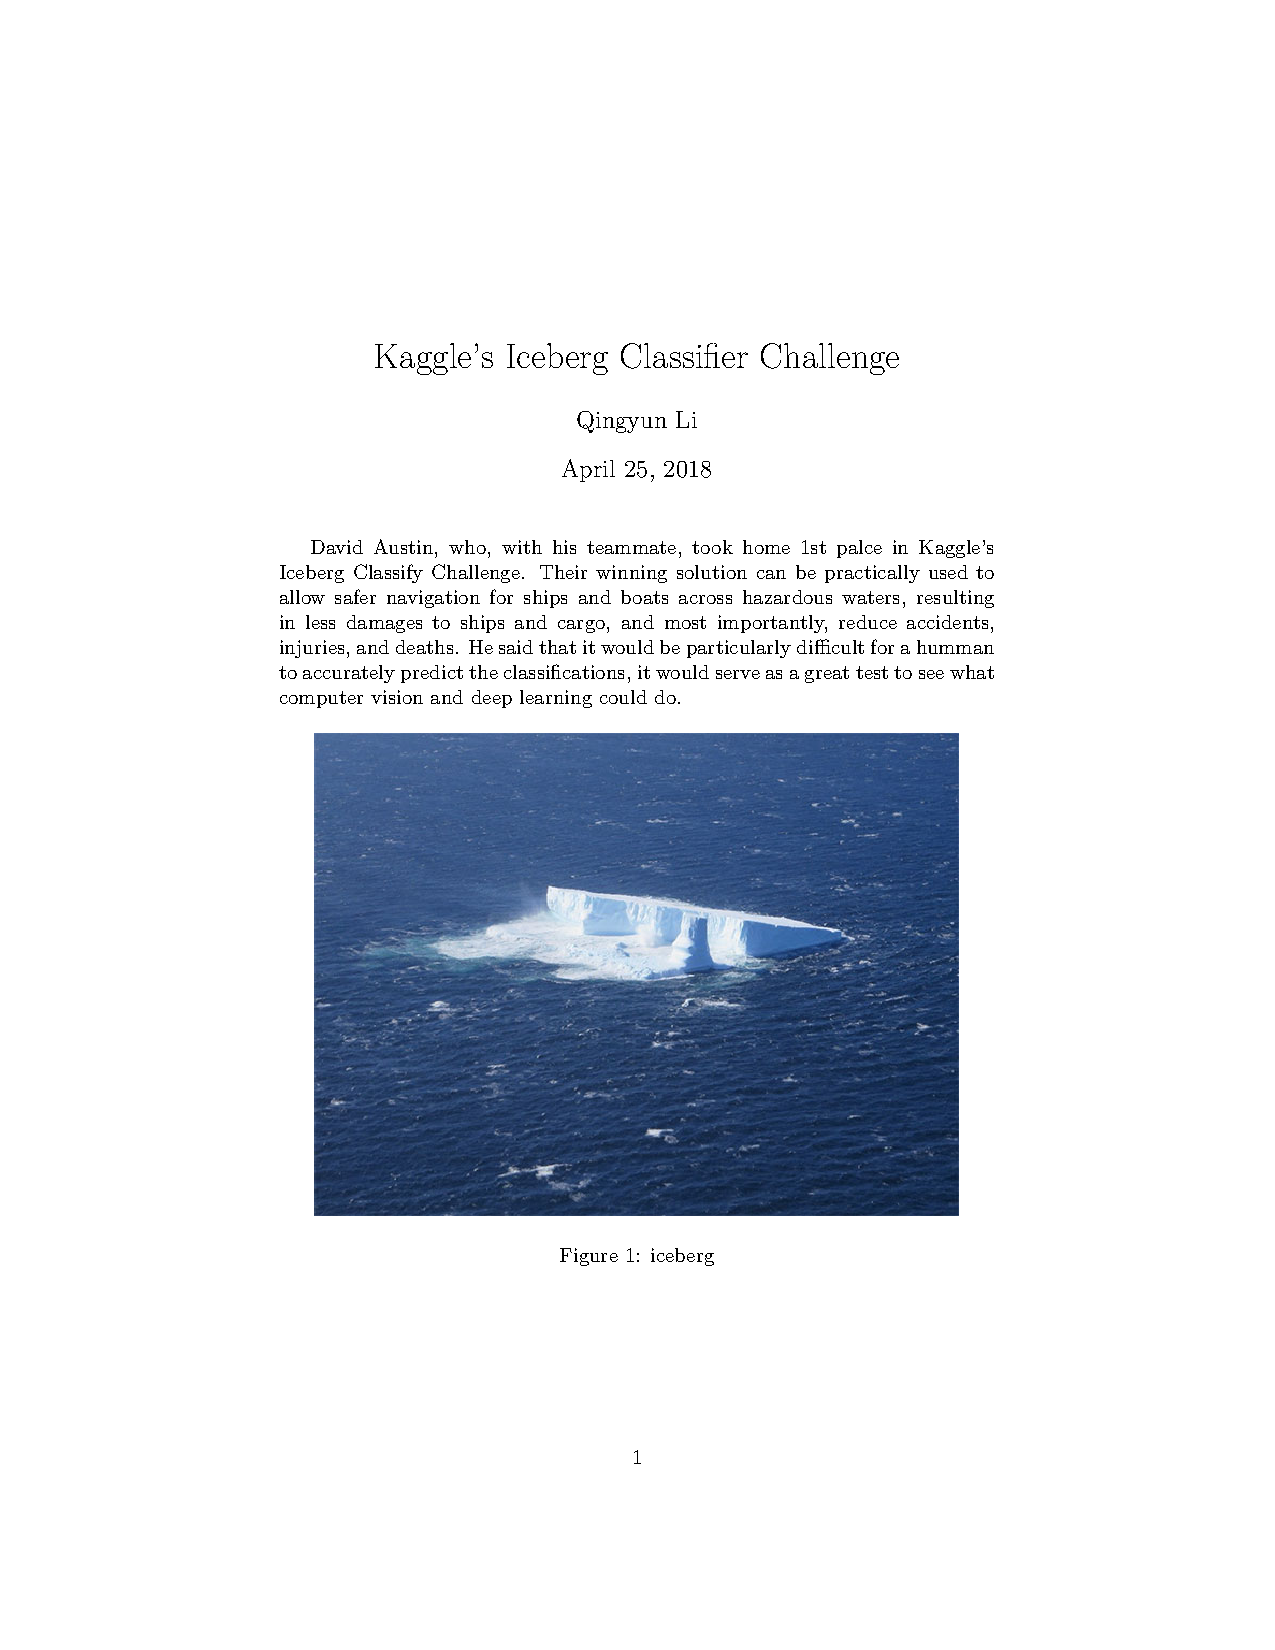
\includegraphics[width=0.9\linewidth]{iceberg.png}\\
\caption{iceberg}\label{image} 
\end{minipage}
\end{figure}
\end{document}